\newpage
\hypertarget{}{}
\section{Tree To Text}
\genHeader

All new, coming soon -- applies for BOTH!

Final step to converting model to text, or doing a complete loop in bidirectional transformation! wait, does this apply to everybody? I think it does!

\begin{itemize}

\item[$\blacktriangleright$] Yay! Almost time to partyParty. Now we work with the parser! Transform our created tree into actual text. (if you look at the
\texttt{out} content files : still empty) \ldots copy paste some content from prev.

\item[$\blacktriangleright$] navigate to ``src/org.moflon.moca.dictionary.unparser'' and open \texttt{DictionaryTreeParser.g}. Edit the contents as
depicted below

\begin{figure}[htp]
\begin{center}
  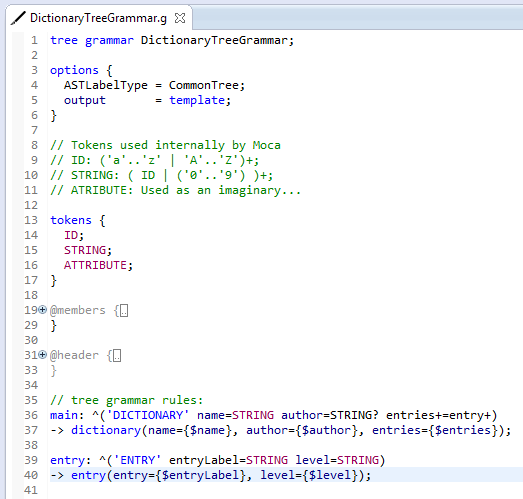
\includegraphics[width=\textwidth]{eclipse_dictionaryTreeGrammar}
  \caption{figureCaption}
  \label{eclipse:treeGrammar}
\end{center}
\end{figure}

In the same folder, check out the generated \texttt{DictionaryUnparserAdapter.java}, a method for retrieving a group of templates
has to be implemented (Approximately line: 40) fig! It has some comments that explain..

\item[$\blacktriangleright$] small example means single file ideal. Remove everything but line 43 so that your file now resembles.. (see orig for now)
for now)

\item[$\blacktriangleright$] Awesome! Now we actually have to create THAT template group. Navigate to the empty ``templates'' folder and create a new file
called \texttt{Dictionary.stg}. Edit it with the stuff from FIG below.


\begin{figure}[htp]
\begin{center}
  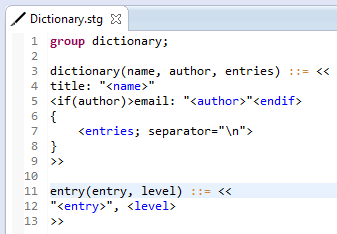
\includegraphics[width=\textwidth]{eclipse_dictionaryTemplate}
  \caption{figureCaption}
  \label{eclipse:dictionaryTemplate}
\end{center}
\end{figure}

\item[$\blacktriangleright$] Open \texttt{MocaMain} in ``org.moflon.moca'' once again and confirm the \emph{unparse} command is present. Uncomment line 24,
which you removed at the start.

\item[$\blacktriangleright$] Run this file - you should now have the same content in both your input and output files!

\end{itemize}